%\chapter{det-comp}

\fixme{NOTE FOR APA Reviewers:  This document is an excerpt from the forthcoming ProtoDUNE-SP TDR, to be submitted to CERN later in 2016.  The draft is still in development. }
%%%%%%%%%%%%%%%%%%%%%%%%%%%%%%%%%%%%%%%%%%%%%%
\section{Anode Plane Assemblies}

Anode Plane Assemblies (APAs) are the detector elements utilized to sense ionization created by charged particles traversing the liquid argon volume inside the single-phase TPC.  ProtoDUNE-SP will feature six APAs, arranged in two rows of three, flanking either side of a central cathode plane.  This section describes the initial physics requirements that drive the APA design parameters, and provides a complete description of APA construction and testing procedures.

\fixme{testing prior to installation?}

%%%%%%%%%%%%%%%%%%%%%%%%%%
\subsection{Scope, requirements, design parameters}

\fixme{start with scope?}

%%%%%%%%%%%%
\subsubsection{Requirements - listing of basic physics requirements}

The initial physics performance requirements that drive the design of the APA are listed in Table \ref{tab:physicsrequirements}.  These are chosen to enable ProtoDUNE-SP to perform high-efficiency reconstruction throughout the entire active volume of the LArTPC, across the broad range of particle momenta and species present in the beam.  

% was cc, changed to lr
\begin{cdrtable}[APA Physics Requirements]{lr}{physicsrequirements}{Preliminary physics requirements that motivate APA design parameters.}   
Requirement & Value  \\ \toprowrule
MIP Identification & 100$\%$ efficiency \\ \colhline
High efficiency for charge reconstruction & $>$90$\%$ for $>$100 MeV \\ \colhline
Vertex Resolution (x,y,z) & (1.5 cm, 1.5 cm, 1.5 cm)\\ \colhline
\textbf{Particle Identification} & \\ 
Muon Momentum Resolution & $<$18$\%$ for non-contained \\
            & $<$5$\%$ for contained\\ 
Muon Angular Resolution & $<$1$^{\circ}$\\            
Stopping Hadrons Energy Resolution & 1-5$\%$\\
Hadron Angular Resolution & $<$10$^{\circ}$ \\ \colhline
\textbf{Shower identification} & \\
Electron efficiency & $>$90$\%$\\
Photon mis-identification & $<$1$\%$\\
Electron Angular Resolution & $<$1$^{\circ}$ \\
Electron Energy Scale Uncertainty & $<$5$\%$\\
\end{cdrtable}

The ability to identify minimum-ionizing particles (MIPs) is a function of several detector parameters, including: argon purity, drift distance, diffusion, wire pitch, and ENC.  ProtoDUNE-SP requires that MIPs originating anywhere inside the active volume of the detector be reconstructed with 100$\%$ efficiency.   The choice of wire pitch (i.e., $\sim$5 mm), combined with the design values of the other parameters just mentioned (and described in their respective sections of the TDR), should enable this 100$\%$ efficiency to be achieved for MIPs.
\fixme{added ENC to acronyms-vol2; need to define it}

\fixme{I had trouble getting the gist of this next pgraph; please see rewrite below it}
Precisely identifying the location of any vertices in an event (e.g., the primary vertex in a neutrino interaction, or gamma conversion points in a $\pi^{0}$ decay) has direct impact on reconstruction efficiency.  The fine granularity of the LArTPC enables excellent performance in this task.  ProtoDUNE-SP requires a vertex resolution such that the fiducial volume, which among other factors determines the number of target nucleons that is a component in cross section measurements, in an analysis can be determined to $<$1$\%$.  This translates into a vertex resolution of $\sim$1.5 cm along each coordinate direction.  In practice, the resolution on the drift-coordinate ($x$) of a vertex/hit will be better than the resolution on its location in the $y-z$ plane, originating from the combination of drift-velocity and electronics sampling-rate.
%\fixme{double-check these vertex numbers, which are very likely incorrect at the moment.}

\fixme{rewrite of above pgraph; if ok please delete previous paragraph} 
The fine granularity of the LArTPC enables excellent precision in identifying the location of any vertices in an event (e.g., the primary vertex in a neutrino interaction, or gamma conversion points in a $\pi^{0}$ decay), which has a direct impact on reconstruction efficiency. ProtoDUNE-SP requires that it be possible to determine the fiducial volume (via analysis) to $<$1$\%$ in order to reach a vertex resolution of $\sim$1.5 cm along each coordinate direction. (The fiducial volume, among other factors, determines the number of target nucleons, which is a component in cross section measurements.) In practice, the resolution on the drift-coordinate ($x$) of a vertex or hit will be better than that on its location in the $y-z$ plane, due to the combination of drift-velocity and electronics sampling-rate.


%%%%%%%%%%%%
\subsubsection{Overall physical description - connection to requirements.}

Figure \ref{fig:tpc_apa1} depicts a diagram of a ProtoDUNE-SP APA.  Each side of an APA consists of three layers of sense wires, plus additional grid and mesh layers.  Collection plane wires (labeled ``X'') span vertically from the bottom of the APA to the top.  There are two planes of induction wires (labeled ``U'' and ``V'') that wrap in a helical fashion, around the long edge of the APA, from the bottom of the APA to the top.  A grid layer (labeled ``G'') also spans from the bottom of the APA to the top, and is not connected for electronic readout.  The mesh layer (labeled ``M'') is secured directly to the APA frame, and effectively defines an equipotential plane over the entire surface area of the frame.  The arrangement of all layers, from the outside-in, is G-U-V-X-M. 

\fixme{rewrite above pgraph}
Figure \ref{fig:tpc_apa1} depicts ProtoDUNE-SP APA, each  side of which consists of three layers of sense wires, plus additional grid and mesh layers.  All wire layers span the entire area of the APA frame. Collection plane wires (labeled ``X'') run vertically.  Two planes of induction wires (labeled ``U'' and ``V'') wrap in a helical fashion around the long edge of the APA.  A grid layer (labeled ``G'') also spans the APA's length, but is not connected for electronic readout.  The mesh layer (labeled ``M'') is secured directly to the APA frame, and effectively defines an equipotential plane over the entire surface area of the frame.  The ordering of the layers, from the outside-in, is G-U-V-X-M. 

\begin{cdrfigure}[APA Diagram]{tpc_apa1}{Sketch of a ProtoDUNE-SP APA. The frame with portions of three wire layers: X is dark blue, V is magenta and U is green.  All layers fill the entire frame area.  There is fourth layer, the G or grid layer, in which the wires run parallel to the X layer.}
\includegraphics[width=0.8\textwidth, angle=90]{figures/tpc_apa1.png} 
\end{cdrfigure}

\fixme{Rewrite of fig caption: Sketch of a ProtoDUNE-SP APA. This shows only portions of each of the three wire layers, U (green), V (magenta) and X (blue), to accentuate their angular relationships to the frame and to each other.  All layers actually span the entire APA frame area on both sides of the APA structure. The induction layers (U and V) are connected electrically across both sides.  The wires in the grid layer, G (not shown), run vertically, parallel to the X layer wires. (What about M?)}

Table \ref{tab:apaparameters} lists some of the high-level parameters of the APA design.

% changed cc to lr
\begin{cdrtable}[APA Design Parameters]{lr}{apaparameters}{APA Design Parameters.}   
Parameter & Value  \\ \toprowrule
Active Height & 5.920 m\\ \colhline
Active Width & 2.295 m\\ \colhline
Wire Pitch (U,V) & 4.67 mm\\ \colhline
Wire Pitch (X,G) & 4.79 mm\\ \colhline
Wire Position Tolerance & 0.5 mm \\ \colhline
Wire Plane Spacing & 5 mm\\ \colhline
Wire Angle (w.r.t. vertical) (U,V) & 35.7$^{\circ}$\\ \colhline
Wire Angle (w.r.t. vertical) (X,G) & 0$^{\circ}$\\ \colhline
Number Wires / APA & 960 (X), 960 (G), 800 (U), 800 (V) \\ \colhline
Number Electronic Channels / APA & 2560 \\ \colhline
Wire Tension & 5.0 N \\ \colhline
Wire Material & Beryllium Copper \\ \colhline
Wire Diameter & 150 $\mu$m \\ \colhline
Wire Resistivity & 7.68 $\mu\Omega$-cm $@$ 20$^{\circ}$ C \\ \colhline
Wire Resistance/m & 4.4 $\Omega$/m $@$ 20$^{\circ}$ C \\ \colhline
Frame Planarity & 5 mm \\ \colhline
Photon Detector Slots & 10 \\
\end{cdrtable}


The APA layers are listed in Table \ref{tab:bias}, along with their operating voltages.  When operated at these voltages, the drifting ionization follows trajectories around the grid and induction wires, ultimately terminating on a collection plane wire; i.e., the grid and induction layers are completely transparent to drifting ionization, and the collection plane is completely opaque.  The grid layer is present for pulse-shaping purposes, effectively shielding the first induction plane from the drifting charge and removing the long leading edge from the signals on that layer; again, it is not connected to the electronics readout. The mesh layer serves to shield the sense planes from pickup from the Photon Detection System and  from ``ghost'' tracks that would otherwise be created when ionizing particles have a trajectory that passes through the planes.  \fixme{the M layer prevents creation of ghost tracks? or they exist but M shields the sense plates from them?}


\begin{cdrtable}[Baseline bias voltages for APA wire layers]{lr}{bias}{Baseline bias voltages for APA wire layers}   
Anode Plane & Bias Voltage  \\ \toprowrule
Grid (G) & -665 V\\ \colhline
Induction (U) & -370 V\\ \colhline
Induction (V) & 0 V\\ \colhline
Collection (X) & 820 V\\ \colhline
Mesh (M) & 0 V\\
\end{cdrtable}

The wrapped style allows the APAs to tile the active area of the LArTPC, minimizing the amount of dead space occupied by electronics and associated cabling.  The size of the APAs is chosen to be compatible with over-the-road shipping, and eventual transport to the 4850 level at SURF, into the membrane cryostat of a detector module.  The dimensions are also chosen such that an integral number of electronic readout channels and boards will fill in the full area of the APA. The modularity of the APAs allows them to be built and tested at off-site production facilities, decoupling their manufacturing time from the construction of the membrane cryostat.  

In the current design of the single-phase DUNE detector module, a central row of APAs is flanked by  drift-fields, requiring sensitivity on both sides. The wrapped APAs allow the induction plane wires to sense drifting ionization originating from either side of the APA.  This double-sided feature is not strictly necessary for the ProtoDUNE-SP arrangement, which has APAs located against the cryostat walls and a drift field on one side only, but it is compatible with this setup as the grid layer facing the wall effectively blocks any ionization outside the TPC from drifting in to the wires on that side of the APA.

Reconstruction of events recorded by the APAs will need to address ambiguities inherent to the wrapped wire design. This can occur when multiple isochronic hits are recorded, potentially leading to reconstructed hits that cannot be traced to unique wire-crossing positions in the detector.  The angle of the induction planes in the APA ($\pm$35.7$^{\circ}$) is chosen such that each induction wire only crosses a given collection wire one time, reducing the ambiguities that the reconstruction must address.  The design angle of the induction wires, coupled with their pitch, was also chosen such that an integer multiple of electronics boards reads out one APA.


The choices of wire tension and wire placement accuracy are made to ensure proper operation of the LArTPC at voltage, and to provide the precision necessary for reconstruction.  The tension of 5~N, when combined with the intermediate support combs that will be described in the next section, \fixme{specify sec} ensure that the wires are held taught in place with no sag.  Wire sag can impact the precision of reconstruction, as well as the transparency of the TPC.  The tension of 5~N is low enough that when the wires are cooled, which will increase their tension due to thermal contraction, they will stay safely below the break load of the beryllium copper wire, as described in the following section. \fixme{specify sec}  To further mitigate wire breakage and its impact on detector performance, each wire in the APA is anchored twice on both ends, with both solder and epoxy.  Details of this arrangement are provided in the following sections. \fixme{specify sec} 


%\begin{itemize}
%\item{Angle and reason for chosen angle}
%\item{Wire placement accuracy}
%\begin{itemize}
%\item{Wire Tension}
%\item{Double anchor at each wire end}
%\item{Need for intermediate support}
%\begin{itemize}
%\item{Sag prevention}
%\item{Break mitigation}
%\end{itemize}
%\end{itemize}
%\item{Voltage requirements for induction plane transparency.}
%\item{Frame distortion consequences - (Lee G. will update previous study)}
%\item{Trapped volume and bubbles}
%\item{Mesh, reasons for mesh}
%\item{Grounding - (based on input from EE and grounding/shielding group)}
%\end{itemize}





%%%%%%%%%%%%%%%%
\subsection{APA physical description, Meeting requirements, Fabrication}
\fixme{title needs fixing}
%%%%%%%%%%%%
\subsubsection{Wires}

Beryllium copper (CuBe) wire is known for its high durability and yield strength. It is composed of $\sim$98$\%$ copper, approximately 1.9$\%$ beryllium, and a negligible amount of other elements. The DUNE APA wire has a diameter of 150$\mu$m (.006~in), and is strung in varying lengths across the apparatus. Three key properties for usage in the APA are: low resistivity, high tensile or yield strength, and coefficient of thermal expansion suitable for use with the APA's stainless steel frame.

Tensile strength of the wire describes the wire breaking stress (see Table \ref{tab:wire}).  The yield strength is the stress at which the wire starts to take a permanent (inelastic) deformation and is the important limit stress for our usage -- though most specifications give tensile strength.  Fortunately, for the CuBe alloys of interest, the two are fairly close to each other.  Based on the tensile strength of wire purchased from Little Falls Alloy (over 1380~MPa or 200,000~psi), the yield strength will be greater than 1100~MPa.  Given that the stress while in use is around 280~MPa, this leaves a comfortable margin.

The coefficient of thermal expansion (CTE) describes how material expands and contracts with changes in temperature.  The CTEs of CuBe alloy and 304 stainless steel are very similar.  Integrated down to 87~K, they are 2.7e-3 for stainless and 2.9e-3 for CuBe \fixme{find and add reference to bib file} (from study: ``Cryogenic Material Properties Database'' by Marquardt, Le and Radebaugh of NIST).

Since the wire contracts slightly more than the frame during cool-down the wire tension will go up.  If it starts at 5~N the tension will rise to about 5.5~N when everything is cool.  

The change in wire tension during cool-down could also be a concern.  In the worst case, the wire
 cools quickly to 87~K before any significant cooling of the frame  -- a realistic case because of the differing thicknesses.  In the limiting case, with complete contraction of the wire and none in the frame, the tension would be expected to reach $\sim$11.7 N.  This is still well under the $\sim$20 N yield tension.
In practice the cooling will be done gradually to avoid this tension spike as well as other thermal shock to the APA.

\begin{cdrtable}[CuBe wire tensile strength and CTE]{lr}{wire}{Tensile strength and coefficient of thermal expansion (CTE) of beryllium copper (CuBe) wire.}
%\multicolumn{2}{c}{Properties of beryllium copper wire} \\ 
Parameter & Value \\ \toprowrule
Tensile Strength (from property sheets) (psi) & 208,274 \\ \colhline
Tensile Strength (from actual wire) (psi) & 212,530 \\ \colhline
CTE of CuBe, integrated to 87 K (m/m) & 2.9e-3 \\ \colhline
CTE of 304 stainless steel, integrated to 87 K (m/m) & 2.7e-3 \\
\end{cdrtable}

Figure \ref{fig:tpc_apa_wirelengthvsnoise} shows the intrinsic noise behavior in (plain) stainless steel wire and stainless steel wire plated with copper and gold.  The MicroBooNE TPC uses the plated wire, for example.  CuBe wire has very similar electrical properties to the plated stainless steel wire, and the figure indicates the expected intrinsic noise levels for ProtoDUNE-SP induction and collection wires.  These very low levels of noise are an important factor in the choice of CuBe wire for the APAs.

\begin{cdrfigure}[APA Wire Length vs Noise]{tpc_apa_wirelengthvsnoise}{Noise levels in wire as a function of wire length.  CuBe wire is very similar in behavior to stainless steel wire plated with copper and gold (blue line).}
\includegraphics[width=0.9\textwidth]{figures/tpc_apa_wirelengthvsnoise.png} 
\end{cdrfigure}

\fixme{Anne got to here Fri 8/5}


%%%%%%%%%%%%
\subsubsection{APA Frame}


\paragraph{Dimensions}

The stainless steel frame of the APA (Figs. \ref{fig:tpc_apa_framedrawing} and \ref{fig:tpc_apa_framephoto}) is 6.06 m long, not counting electronics and mounting hardware, and 2.30 m wide.  It is 76.2 mm thick, made from imperial size 3 in $\times$ 4 in $\times$ 0.120 in wall rectangular tubing.  The cross pieces are 2 in $\times$ 3 in $\times$ 0.120 in wall tubing.  It will be mounted in the cryostat with its long axis vertical; multiple APAs will be mounted edge to edge to form a continuous plane. An electron deflection technique will be used to ensure that electrons that are drawn towards a joint between two APAs will be deflected to one or the other and not lost.

\begin{cdrfigure}[APA Dimensions]{tpc_apa_framedrawing}{An APA showing overall dimensions and main components.}
\includegraphics[width=0.9\textwidth]{figures/tpc_apa_framedrawing.png} 
\end{cdrfigure}

\begin{cdrfigure}[APA Photograph]{tpc_apa_framephoto}{An APA frame mounted in a transport cart (for moving it from frame fabrication site to APA fabrication site).}
\includegraphics[width=0.9\textwidth]{figures/tpc_apa_framephoto.png} 
\end{cdrfigure}

\paragraph{Welded vs. modular construction}

Early prototypes of the APA frame were welded.

Switching to a modular design, however, has improved dimensional accuracy and ease of fabrication, Figs. \ref{fig:tpc_apa_boltedjointdrawing} and \ref{fig:tpc_apa_boltedjointphoto}.  Welding distortion, particularly distortion that would worsen the flatness of the APA, is time consuming to avoid.  The individual tubes now have threaded pads welded to the ends that are machined flat and square (after welding) so the frame is assembled with machine screws.

Other advantages of this modular construction include easier transportation/shipping of fabricated but unassembled frames and easier and more economical replacement of a frame member if one is found to be defective.

\begin{cdrfigure}[APA Bolted Joint Drawing]{tpc_apa_boltedjointdrawing}{A model of the bolted joint.  The holes on the top of the tube are for access to tighten the screws.  The heads actually tighten against the lower hole, inside the tube.}
\includegraphics[width=0.9\textwidth]{figures/tpc_apa_boltedjointdrawing.png} 
\end{cdrfigure}

\begin{cdrfigure}[APA Bolted Joint Photograph]{tpc_apa_boltedjointphoto}{A fabricated and bolted up joint.}
\includegraphics[width=0.9\textwidth]{figures/tpc_apa_boltedjointphoto.png} 
\end{cdrfigure}

\paragraph{Wire loads}

The many wires strung across the frame, each with a 5 N tension ($\sim$1.1 lb), apply a large, compressive, in-plane load around the perimeter of the APA.  Finite element analysis, Figs. \ref{fig:tpc_apa_distortion} and \ref{fig:tpc_apa_maxstress} has shown that the distortions caused by these loads are small.

\begin{cdrfigure}[APA Distortion]{tpc_apa_distortion}{Distortion of the APA frame under wire load.  Arrows are not shown across end tubes but loading is present as an evenly distributed load.  The maximum in-plane distortion seen with this loading is under 0.2 mm.}
\includegraphics[width=0.9\textwidth]{figures/tpc_apa_distortion.png} 
\end{cdrfigure}

\begin{cdrfigure}[APA Maximum Stress]{tpc_apa_maxstress}{Analysis of maximum stress due to wire load.  The maximum is 52 Mpa.  The yield stress of 304SS is around 240 MPa. (The stated 351.6 MPa is optimistic!)}
\includegraphics[width=0.9\textwidth]{figures/tpc_apa_maxstress.png} 
\end{cdrfigure}

Although the compressive long direction load has raised concern about buckling, that is not an issue here:
\begin{itemize}
\item{The loads at opposite ends do not remain collinear as the frame deforms because the wires are constrained to stay close to the surface of the APA.}
\item{If the frame were to start to bow, tilting of the boards that hold the wires would cause a change in wire tension strongly countering that bowing -- opposite of the increasing sort of effects that lead to buckling.}
\end{itemize}

\paragraph{Other FEA results}

Other FEA studies have been done to verify what hand calculations show -- the APA structure is stiff enough to stay well within allowable deformation and stress limits for any expected load.  A couple of these are shown in Figs. \ref{fig:tpc_apa_distortion_simplesupport}, \ref{fig:tpc_apa_stress_simplesupport}, \ref{fig:tpc_apa_distortion_topcentersupport}, and \ref{fig:tpc_apa_stress_topcentersupport}.

\begin{cdrfigure}[APA Distortion Simply Supported]{tpc_apa_distortion_simplesupport}{Deflection of APA simply supported at ends, flat orientation.}
\includegraphics[width=0.9\textwidth]{figures/tpc_apa_distortion_simplesupport.png} 
\end{cdrfigure}

\begin{cdrfigure}[APA Stress Simply Supported]{tpc_apa_stress_simplesupport}{Stress at center of APA simply supported at ends, flat orientation.}
\includegraphics[width=0.9\textwidth]{figures/tpc_apa_stress_simplesupport.png} 
\end{cdrfigure}

\begin{cdrfigure}[APA Distortion Top Center Support]{tpc_apa_distortion_topcentersupport}{Deflection of APA under its own weight hanging from top center.}
\includegraphics[width=0.9\textwidth]{figures/tpc_apa_distortion_topcentersupport.png} 
\end{cdrfigure}

\begin{cdrfigure}[APA Stress Top Center Support]{tpc_apa_stress_topcentersupport}{Stress in APA under its own weight hanging from top center.}
\includegraphics[width=0.9\textwidth]{figures/tpc_apa_stress_topcentersupport.png} 
\end{cdrfigure}

\paragraph{Frame Handling}

All handling of APAs in the factory will be with the long 6 m axis of the APAs in a horizontal plane. Most stations are oriented so that the head end is toward the south, avoiding the large floor space usage that would be required if rotating APAs end for end between one station and another. 

Initially (through ProtoDUNE-SP), bare frame assembly will be in the main PSL building, while winding and other assembly will occur in the south building. A transport cart has been built and used to move bare frames to the south building. (During volume production for the full scale detectors, frame assembly is planned to occur in the south building.)

Bare frames are mounted in carts used both for transport within the production building and as stands in which many fabrication processes occur, such as installing mesh, comb bases, additional combs, boards, and performing soldering and epoxying. These carts are called process carts. 

The mounting to the process cart is done using interface frames and trunnion kits that are also used in the wire winder. The trunnion kits provide for rotation to various angles about the APA's long 6 m axis, and holding rotation angle.

A small gantry crane and a set of jack stands are used to aid in supporting one end of an APA, while the interface frame at that end is removed and reversed to enable winding the other half of a wire layer, or to allow installing more boards at the foot, or to support the frame in a minimal-deflection state while applying and bonding mesh or boards, or to assemble and disassemble the large mesh application jig. 

A large gantry crane is used to move the APA in progress, along with its attached interface frames and trunnion kits, between a process cart and the winder. The rigging equipment used for this move is the vertical rigging kit, a 2-level whiffle tree of spreaders for vertical compactness compared to slings, to make best use of limited hook height and to load the frame at 4 attachment points to manage stresses in the thin tube walls of the APA frame. 

Another rigging kit, the ``H spreader'', enables lifts when the wire planes are horizontal, such as for loading into or removing from a cold test. Formed feet have been designed for minimal tube wall stress when supporting an APA during jack stand use or in a cold test. A storage rack designed to be stable when holding up to 4 APAs in any combination of stations has been built for temporary storage of work in progress.

When the APA is mounted in the winding machine, for applying wire to its surface, it must be mounted so that its long axis is horizontal and so that it can be rotated about that axis.  Although winding will always be done with the APA in ``landscape'' position, there are other tasks that require it to be rotated to a horizontal position (APA surface parallel to ground).

In order to hold it securely in both positions and allow rotation between the two positions an ``interface frame'' set (Fig. \ref{fig:tpc_apa_interfaceframes}) has been designed that connects to the head and foot of the APA.  It has trunnions at each end so the APA/interface frame assembly can be supported in bearings.  This interface frame attaches to the APA in such a way that slightly more than half of the width of each end is exposed for winding of wires.  After half a wire layer is wound the APA is switched so that the interface frame connects to the opposite side and the rest of the APA can be wound.

\begin{cdrfigure}[APA Interface Frames]{tpc_apa_interfaceframes}{A Solidworks model of the interface frames attached to the APA. Trunnions, for mounting in the winding machine, are visible at the ends. Note that the frame is exposed for winding at the tail (top image) end and a temporary toothed board is similarly exposed at the head (bottom image) end.}
\includegraphics[width=0.9\textwidth]{figures/tpc_apa_interfaceframes.png} 
\end{cdrfigure}

\paragraph{Effect on in-plane wire spacing of in-plane frame deviations.}

The effect of in-plane frame deviations is straight forward.  If features that locate a wire move in a direction parallel to the wire, the wire position is unaffected. If they move perpendicular to the wire then the end of the wire is moved by the same amount -- with a diminishing effect along the wire away from that point.  

Minimizing in-plane deviations hinges on accurate machining of the APA component parts.  If the mounting holes for wire guide boards on the tubes are accurately placed, and if the joining surfaces between tubes are accurately machined, and then if the wire guide boards themselves are accurately machined, these distortions will be minimized.  The deviations in wire position will be similar magnitude to the machining deviations.

\paragraph{Effect on layer spacing of the out-of-plane frame deviations.}

In-plane distortions only affect the spacing between wires within a plane.  Out-of-plane distortions are more serious because they affect the spacing between wire planes.  If the spacing is too far from its design value, electrons will be absorbed at induction layers -- a loss of transparency.  Calculations have shown that, although a millimeter or more of layer plane spacing change can be accommodated by adjusting the wire layer voltages, our goal is to keep the layer spacing accurate to within 0.5 mm.

Calculations have been done to show the effect on wire plane spacing of several basic distortions in the APA frame.  The distortions studied were: a twist, a bow along the length, and a fold down the middle (Figs. \ref{fig:tpc_apa_twistdistortion}, \ref{fig:tpc_apa_bowdistortion}, and \ref{fig:tpc_apa_folddistortion}).  (A fold between the top half and the bottom half is considered unlikely and a bow across the width would be similar to, but slightly less severe than, the lengthwise fold so these three should be able to approximate a general distortion.)

Although the APA is 6 m long, it's divided into 5 cells by the steel cross members of the frame.  There is a series of ``combs'' along each of these cross members that maintains in-plane and out-of-plane spacing.  This isolates deviations in wire spacing in one cell from deviations in the others and means that the wire spacing around the edges of these cells is as accurate as the machining of the combs and wire boards bordering the cells.  We looked at the wire plane spacing effect of the above distortions within a cell and then related that to the distortions of the entire frame.

\begin{cdrfigure}[APA Twist Distortion]{tpc_apa_twistdistortion}{A sketch of the ``twist'' distortion of magnitude ``a''.  One of the five cells of an APA is shown here.}
\includegraphics[width=0.9\textwidth]{figures/tpc_apa_twistdistortion.png} 
\end{cdrfigure}

\begin{cdrfigure}[APA Bow Distortion]{tpc_apa_bowdistortion}{A sketch of the ``bow'' distortion.}
\includegraphics[width=0.9\textwidth]{figures/tpc_apa_bowdistortion.png} 
\end{cdrfigure}

\begin{cdrfigure}[APA Fold Distortion]{tpc_apa_folddistortion}{A sketch of the ``lengthwise fold'' distortion.}
\includegraphics[width=0.9\textwidth]{figures/tpc_apa_folddistortion.png} 
\end{cdrfigure}

For each out-of-plane distortion considered we calculated the deformation of the wire planes and then compared adjacent planes to find the change in wire plane spacing over the entire cell.  This gave plots such as Fig. \ref{fig:tpc_apa_wirespacingchange}.  Looking for the worst effect among the sets of adjacent layers gave us the limits on frame distortion.  We scaled those distortions to give the maximum magnitude of each of these distortions for a 0.5 mm change in wire plane spacing.
Fortunately, the three distortions considered have their largest effect on the wire layers in 3 different locations so each of the distortions can be considered separately.  This means if the distortion of a frame is considered as the sum of the three distortion modes, their effect is fairly independent.

\begin{cdrfigure}[APA Wire Plane Spacing Change]{tpc_apa_wirespacingchange}{A plot of wire plane spacing change.}
\includegraphics[width=0.9\textwidth]{figures/tpc_apa_wirespacingchange.png} 
\end{cdrfigure}

Detail is shown in the technical report ``Layer Distortion Summary 6m Frame.pptx''.
The net results are as follows.  A 0.5 mm change in wire plane spacing could come from:
\begin{itemize}
\item{6 mm overall out-of-flatness in the frame due to twist (1 mm/m of frame length)}
\item{11 mm out-of-flatness due to bow}
\item{1.2 mm out-of-flatness due to a ``fold'' down the center}
\end{itemize}
    
This is proportional so that 12 mm of twist, or 22 mm of bow, or 2.4 mm of fold would cause a 1.0 mm change in wire plane spacing.

\paragraph{Measured deviation in fabricated frame geometry}

The prototype frame that has been constructed to test the APA fabrication process (the ``process  prototype'') has been surveyed to measure its deviation from ``perfect'' geometry.  This was done with retroreflectors and a Leica TCRA1201+ theodolite (Fig. \ref{fig:tpc_apa_framesurveyphoto}).

\begin{cdrfigure}[APA Frame Survey Photograph]{tpc_apa_framesurveyphoto}{Modular frame being surveyed after fabrication.}
\includegraphics[width=0.9\textwidth]{figures/tpc_apa_framesurveyphoto.png} 
\end{cdrfigure}

The two main categories of data are in-plane and out-of-plane distortions. The plot in Fig. \ref{fig:tpc_apa_framesurvey_inplane} shows the in-plane distortion measured in this frame.

\begin{cdrfigure}[APA Frame Survey In-Plane Distortions]{tpc_apa_framesurvey_inplane}{Plot of in-plane deviations.}
\includegraphics[width=0.9\textwidth]{figures/tpc_apa_framesurvey_inplane.png} 
\end{cdrfigure}

The blue dots in Fig. \ref{fig:tpc_apa_framesurvey_inplane} show the theoretical locations of several points on the frame; the axes give positions in meters.  The other set of dots, the orange ones, show the deviation from perfect position.  If there were no deviation the points would be on top of each other; the greater the space between the theoretical and measured points the greater the deviation from perfect.  In this plot the same scale is used on the side except that the scale now represents millimeters.  So, a point that is measured to be in error by a mm is plotted, in the correct direction, a millimeter (on the plot scale) from the perfect point.

\begin{cdrfigure}[APA Frame Survey Out-of-Plane Distortions]{tpc_apa_framesurvey_outplane}{Plot of out-of-plane deviations in the measured process prototype.  The deviations range from a low of -2.14 mm to a high 1.35 for a total out of flatness of 3.5 mm.}
\includegraphics[width=0.9\textwidth]{figures/tpc_apa_framesurvey_outplane.png} 
\end{cdrfigure}

The plot in Fig. \ref{fig:tpc_apa_framesurvey_outplane} shows the measured out-of-plane deviations.  To avoid out-of-plane distortion of the frame by gravity the frame was held for survey by two points along the bottom rail and by one point near the top edge that kept it from falling over (Fig. \ref{fig:tpc_apa_framesurveyphoto}) but was not tight enough to twist or bend the member to which it attached.  All of the points on the measured surface fall between two planes 3.5 mm apart.

\begin{cdrfigure}[APA Frame Survey Locations]{tpc_apa_framesurvey_locations}{Locations along length of APA in displacement tables.}
\includegraphics[width=0.9\textwidth]{figures/tpc_apa_framesurvey_locations.png} 
\end{cdrfigure}

\begin{cdrtable}[APA Survey Data]{cccc}{apasurvey}{Out of plane displacements at survey points.}
right & center & left &  \\ \toprowrule
-0.71067 & 0.674997 & 1.289473 & Foot tube \\ \colhline
-1.22419 & -0.41287 & 1.224186 & Pt. 1  \\ \colhline
-0.64366 & -0.71188 & -0.08949 & Pt. 2  \\ \colhline
-0.11308 & -0.98559 & -0.80455 & Pt. 3  \\ \colhline
1.001953 & -0.84197 & -1.60603 & Pt. 4  \\ \colhline 
1.345262 & -0.65297 & -2.14083 & Pt. 5  \\ \colhline
1.224186 & -0.4957 & -1.22419 & Pt. 6  \\ \colhline
0.603007 & 0.085745 & -0.43262 & Head tube \\
\end{cdrtable}

\begin{cdrfigure}[APA Frame Calculated Distortion]{tpc_apa_calculateddistortion}{The three calculated distortion values: twist in each one of the five cells, overall bow, and fold at each of the cross bars.}
\includegraphics[width=0.9\textwidth]{figures/tpc_apa_calculateddistortion.png} 
\end{cdrfigure}

Fig. \ref{fig:tpc_apa_framesurvey_locations} shows the points that were surveyed for out-of-plane location on the APA and table \ref{tab:apasurvey} shows the results.  This data was used to calculate the twist in each cell as shown in Fig.  \ref{fig:tpc_apa_calculateddistortion}. The measured twist in each cell is shown; the allowable twist (for a 0.5 mm wire plane spacing change) is greater than any of these.  The overall bow is shown in Fig. \ref{fig:tpc_apa_calculateddistortion}; the allowable is greater than this.  The fold at each cross bar is shown in Fig. \ref{fig:tpc_apa_calculateddistortion} and, again, the allowable is greater than any of the measured values.



%%%%%%%%%%%%
\subsubsection{Wire and Wire Wrapping}

\paragraph{Geometry}

Each side of the APA frame is covered with four layers of wires.  Fig. \ref{fig:tpc_apa_cornerphoto} shows a corner of the APA and the four layers

\begin{cdrfigure}[APA Corner Photograph]{tpc_apa_cornerphoto}{Corner of an APA.  The wires in the first and fourth layers on each side are parallel to the long axis of the APA.  The second and third layers are angled at 35.7$^{\circ}$ to this axis, angled in opposite directions to each other.}
\includegraphics[width=0.9\textwidth]{figures/tpc_apa_cornerphoto.png} 
\end{cdrfigure}

All the wires start at the top end (right hand end in fig. \ref{fig:tpc_apa1}) of the APA and stop at the bottom. The 1st and 4th layers go straight; the 2nd and 3rd wrap around the sides.

During fabrication wires are wound around the bottom and the top without break.  Wire segments at the top and bottom are snipped out after winding to create individual wires.  This continuous winding process is more efficient than stopping to solder, trim and restart each wire as it's placed.

There are ten stacks of wire boards across each side at the head of the APA.  The X layer board in each stack has room for 48 wires, the V layer has 40 wires, the U layer 40 wires and the G layer 48.  Each board stack, therefore, has 176 wires but only X, V and U are signal layers so there are 128 signal channels in each stack.  With a total of 20 stacks per APA there are 3520 wires starting at the top of the APA and ending at the bottom.  This is a total of $\sim$23.4 km of wire on the surfaces of each APA.

The 128 signal channels in each board stack means 2560 signal channels per APA.

\paragraph{Side and foot boards}

The boards along the sides and foot of the APA have notches, pins or other location features to hold the wires in the correct position as they wrap around the edge from one side of the APA to the other.

G10 circuit board material is ideal for these side and foot boards for its physical properties alone but it has an additional advantage.  There are a number of hole or slot features in the edge boards providing access to the underlying frame.  In order that these openings are not covered by wires the sections of wire that would go over the openings are replaced by traces on the boards.  After the wires are wrapped, the wires over the opening are soldered to pads at the ends of the traces and the section of wire between the pads snipped out (Fig. \ref{fig:tpc_apa_sideboardmodel}).  These traces are easily and economically added to the boards by the many commercial fabricators who make circuit boards.

\begin{cdrfigure}[APA Side Board Model]{tpc_apa_sideboardmodel}{Model of board with wires showing how traces connect wires around openings in the side boards.  The wires are wound straight over the openings, then soldered to pads at the ends of the traces.  After soldering the sections between the pads are trimmed away.}
\includegraphics[width=0.9\textwidth]{figures/tpc_apa_sideboardmodel.png} 
\end{cdrfigure}

Originally, notches were machined into the circuit boards but this was labor intensive.  An alternate method has been developed based on the injection molding of strips with the required notch or pin features and then bonding these strips to the edge of the circuit boards as shown in Fig. \ref{fig:tpc_apa_sideboardphoto}.

\begin{cdrfigure}[APA Side Board Photo]{tpc_apa_sideboardphoto}{Boards with injection molded tooth strips glued on.  The left shows an end board with teeth for locating the longitudinal wires.  The teeth there form small notches. The right is a side board for locating the angled wires where the wires are angled around a pin.}
\includegraphics[width=0.9\textwidth]{figures/tpc_apa_sideboardphoto.png} 
\end{cdrfigure}

The angled wires are located by pins as shown in the right-hand picture of Fig. \ref{fig:tpc_apa_sideboardphoto}.  The wires make a partial wrap around the pin is they change direction from the face of the APA to the edge.  The longitudinal wires aren't pulled to the side so they can't be pulled against a pin.  They are located by teeth with slots as shown in the left-hand picture in Fig. \ref{fig:tpc_apa_sideboardphoto}. 
	
The polymer used for the strips is Vectra e130i (a trade name for 30$\%$ glass filled liquid crystal polymer or LCP). It retains its strength at cryogenic temperature and has a CTE similar enough to G10 that differential expansion/contraction is not a problem.

\paragraph{Glue and solder}
The ends of the wires are soldered to pads on the edge or wire boards.  Solder provides both an electrical connection and a physical anchor to the wires.  As an additional physical anchor the wires are glued for roughly 10 mm near the solder pads.  For example, in Fig. \ref{fig:tpc_apa_sideboardphoto}, in addition to soldering the wires upon the pads shown on the left-hand photograph, an epoxy bead will be applied on top of all wires in the area between the solder pads and the injection molded tooth strips.

2216 gray epoxy by 3M was chosen for the glue.  It is strong, widely used (therefore much data is available), and it retains good properties at cryogenic temperatures.  A 62$\%$ tin, 36$\%$ lead and 2$\%$ silver solder was chosen.  A eutectic mix (63/37) is the best of the straight tin/lead solders but the 2$\%$ added silver gives better creep resistance.

Tests showed that 3 mm long solder pads were not long enough to hold well so the pad length has been increased to 7 mm.  Increasing the cure time (and/or cure temperature) ensures that the glue develops its full strength.  With these modifications good glue and solder holding has been obtained.  Fig. \ref{fig:tpc_apa_creepdata} shows the results of long term tests performed in which wires were constrained by glue, solder or both and their tensions measured over time. (Note: The wobbly traces came from an experimental problem with measuring tension in some of the wires.)  There is some tension loss over time but the key feature to this plot is that all the wires, glue only, solder only, or glue and solder lost tension at the same rate.  If the joints were slipping it would be highly unlikely that the glue only, solder only and both together joints would all slip at the same rate.  This means that the joints are not slipping but, instead, there is stress relaxation in the wires.

Indeed, CuBe wire is known to exhibit some stress relaxation.  The plot in fig. \ref{fig:tpc_apa_creepdata} shows that over 430 days the wire samples (initially tensioned to 10 N, twice the DUNE APA value) lost around 5$\%$ of their tension.  This does not appear to happen quite linearly; the rate of tension loss decreases over time.  (After the last results were taken it was realized that the warm day without the AC on in the room may have lowered the tensions slightly; these tests are ongoing.)

Interestingly, wire samples with an initial tension of 5 N, the target DUNE APA tension, lost about 4$\%$ over the same time interval -- not much less than the wires tensioned to 10 N. 

These results suggest that using solder alone may be adequate.  However, unless further, conclusive testing confirms this, glue will be used in addition to solder. 

The company that makes the wire, Little Falls Alloy, also makes a wire called ``hard'' which means it has been annealed and mechanically hardened without the heat treatment that would further harden it.  In our tests (see the data for Test 4) the stress relaxation only causes about 1$\%$ tension loss.  Although this is desirable, it comes with a cost; the yield strength is only 10 N or so.  This makes the wire more vulnerable to damage.  The tempered wire, with a yield of 20 N, seems a better choice

\begin{cdrfigure}[APA Tension Creep Data]{tpc_apa_creepdata}{Plots of tension vs. time over 430 days for wire strung at an initial tension of $\sim$10 N.  Three methods of fastening the ends were used as shown.}
\includegraphics[width=0.9\textwidth]{figures/tpc_apa_creepdata.png} 
\end{cdrfigure}

\paragraph{Mesh and mesh application}

The mesh layer is glued directly to the steel frame surface -- over the openings in the frame.  It creates a uniform ground layer beneath the wire planes.  In the demonstration 35 ton experiment the APA without mesh showed more noise than the ones with mesh.

The mesh is clamped around the perimeter of the opening and then pulled tight (opening and closing clamps as needed during the process).  When the mesh is taut a 25 mm wide strip is masked off around the opening and glue is applied through the mesh to attach it to the steel.  Although measurements have shown this gives good electrical contact between the mesh and the frame, a deliberate electrical connection will also be made.  Figures \ref{fig:tpc_apa_meshphoto}, and \ref{fig:tpc_apa_meshclampphoto} show the mesh for the 35 ton experiment, while Fig. \ref{fig:tpc_apa_fullsizemeshdrawing} depicts the mesh application setup for a full-size ProtoDUNE-SP APA.

\begin{cdrfigure}[APA Mesh Photo]{tpc_apa_meshphoto}{The mesh in place on a small frame -- with combs.}
\includegraphics[width=0.9\textwidth]{figures/tpc_apa_meshphoto.png} 
\end{cdrfigure}

\begin{cdrfigure}[APA Mesh and Clamps Photo]{tpc_apa_meshclampphoto}{A 35 ton experiment APA with mesh clamped and masked, ready to be glued.}
\includegraphics[width=0.9\textwidth]{figures/tpc_apa_meshclampsphoto.png} 
\end{cdrfigure}

\begin{cdrfigure}[APA Full-Size Mesh Drawing]{tpc_apa_fullsizemeshdrawing}{The mesh clamping jig for the full size APA.}
\includegraphics[width=0.9\textwidth]{figures/tpc_apa_fullsizemeshdrawing.png} 
\end{cdrfigure}

\paragraph{Head Electronics Boards}

The head electronics boards (``wire boards'') are the anchors for the wires at the head end of the APA (Fig. \ref{fig:tpc_apa_wireboardheadphoto}).  They are also the connection between the wires and the data acquisition electronics -- usually called the cold electronics

\begin{cdrfigure}[APA Wire Boards at Head Photo]{tpc_apa_wireboardheadphoto}{The wire boards at the head of one of the 35T APAs.}
\includegraphics[width=0.9\textwidth]{figures/tpc_apa_wireboardheadphoto.png} 
\end{cdrfigure}

At the head end of the APA the wire plane spacing is set by the thickness of these wire boards.  The first layer wires solder to the surface of the first board, the second layer wires to the surface of the second board, etc.  Temporary toothed edge boards beyond these wire boards align and hold the wires until they are soldered to pads on the wire boards.  After soldering the sections going up over the temporary boards are snipped away.

Many of the capacitors and resistors that could be on these wire boards are moved to an auxiliary board (the ``CR board'') to improve their accessibility in case of component failure.  This board rests beneath the wire boards at the top of the frame and links the wire boards to the cold electronics.  The connections between the wire boards and the CR board is made with rows of Mill-Max pins embedded in the wire and CR boards

\paragraph{Modular Electronics}
In the current design (Fig. \ref{fig:tpc_apa_electronicsmountingphoto}), which was used for the 35 ton demo APAs, the cold electronics boards are mounted on a ``fin'' -- a steel plate extending across the width of the APA at the top tube.

\begin{cdrfigure}[APA Electronics Mounting Photo]{tpc_apa_electronicsmountingphoto}{A mockup of the current cold electronics mounting where the cold electronics is mounted on the fin at the head of the APA.}
\includegraphics[width=0.9\textwidth]{figures/tpc_apa_electronicsmountingphoto.png} 
\end{cdrfigure}

A modified design (Fig. \ref{fig:tpc_apa_electronicsmountingdiagram}) is being developed for the ProtoDUNE-SP APAs that consists of small boxes, one near each board stack, that hold the cold electronics for that board stack.  Putting the electronics in small modules simplifies installation and replacement and also helps with the collection of argon gas generated by the warm electronic components.  These modules are mounted in such a way that any of them can be removed from a single side of the APA after APA installation.

\begin{cdrfigure}[APA Electronics Mounting Design]{tpc_apa_electronicsmountingdiagram}{Solid model of revised, modular, cold electronics boxes.}
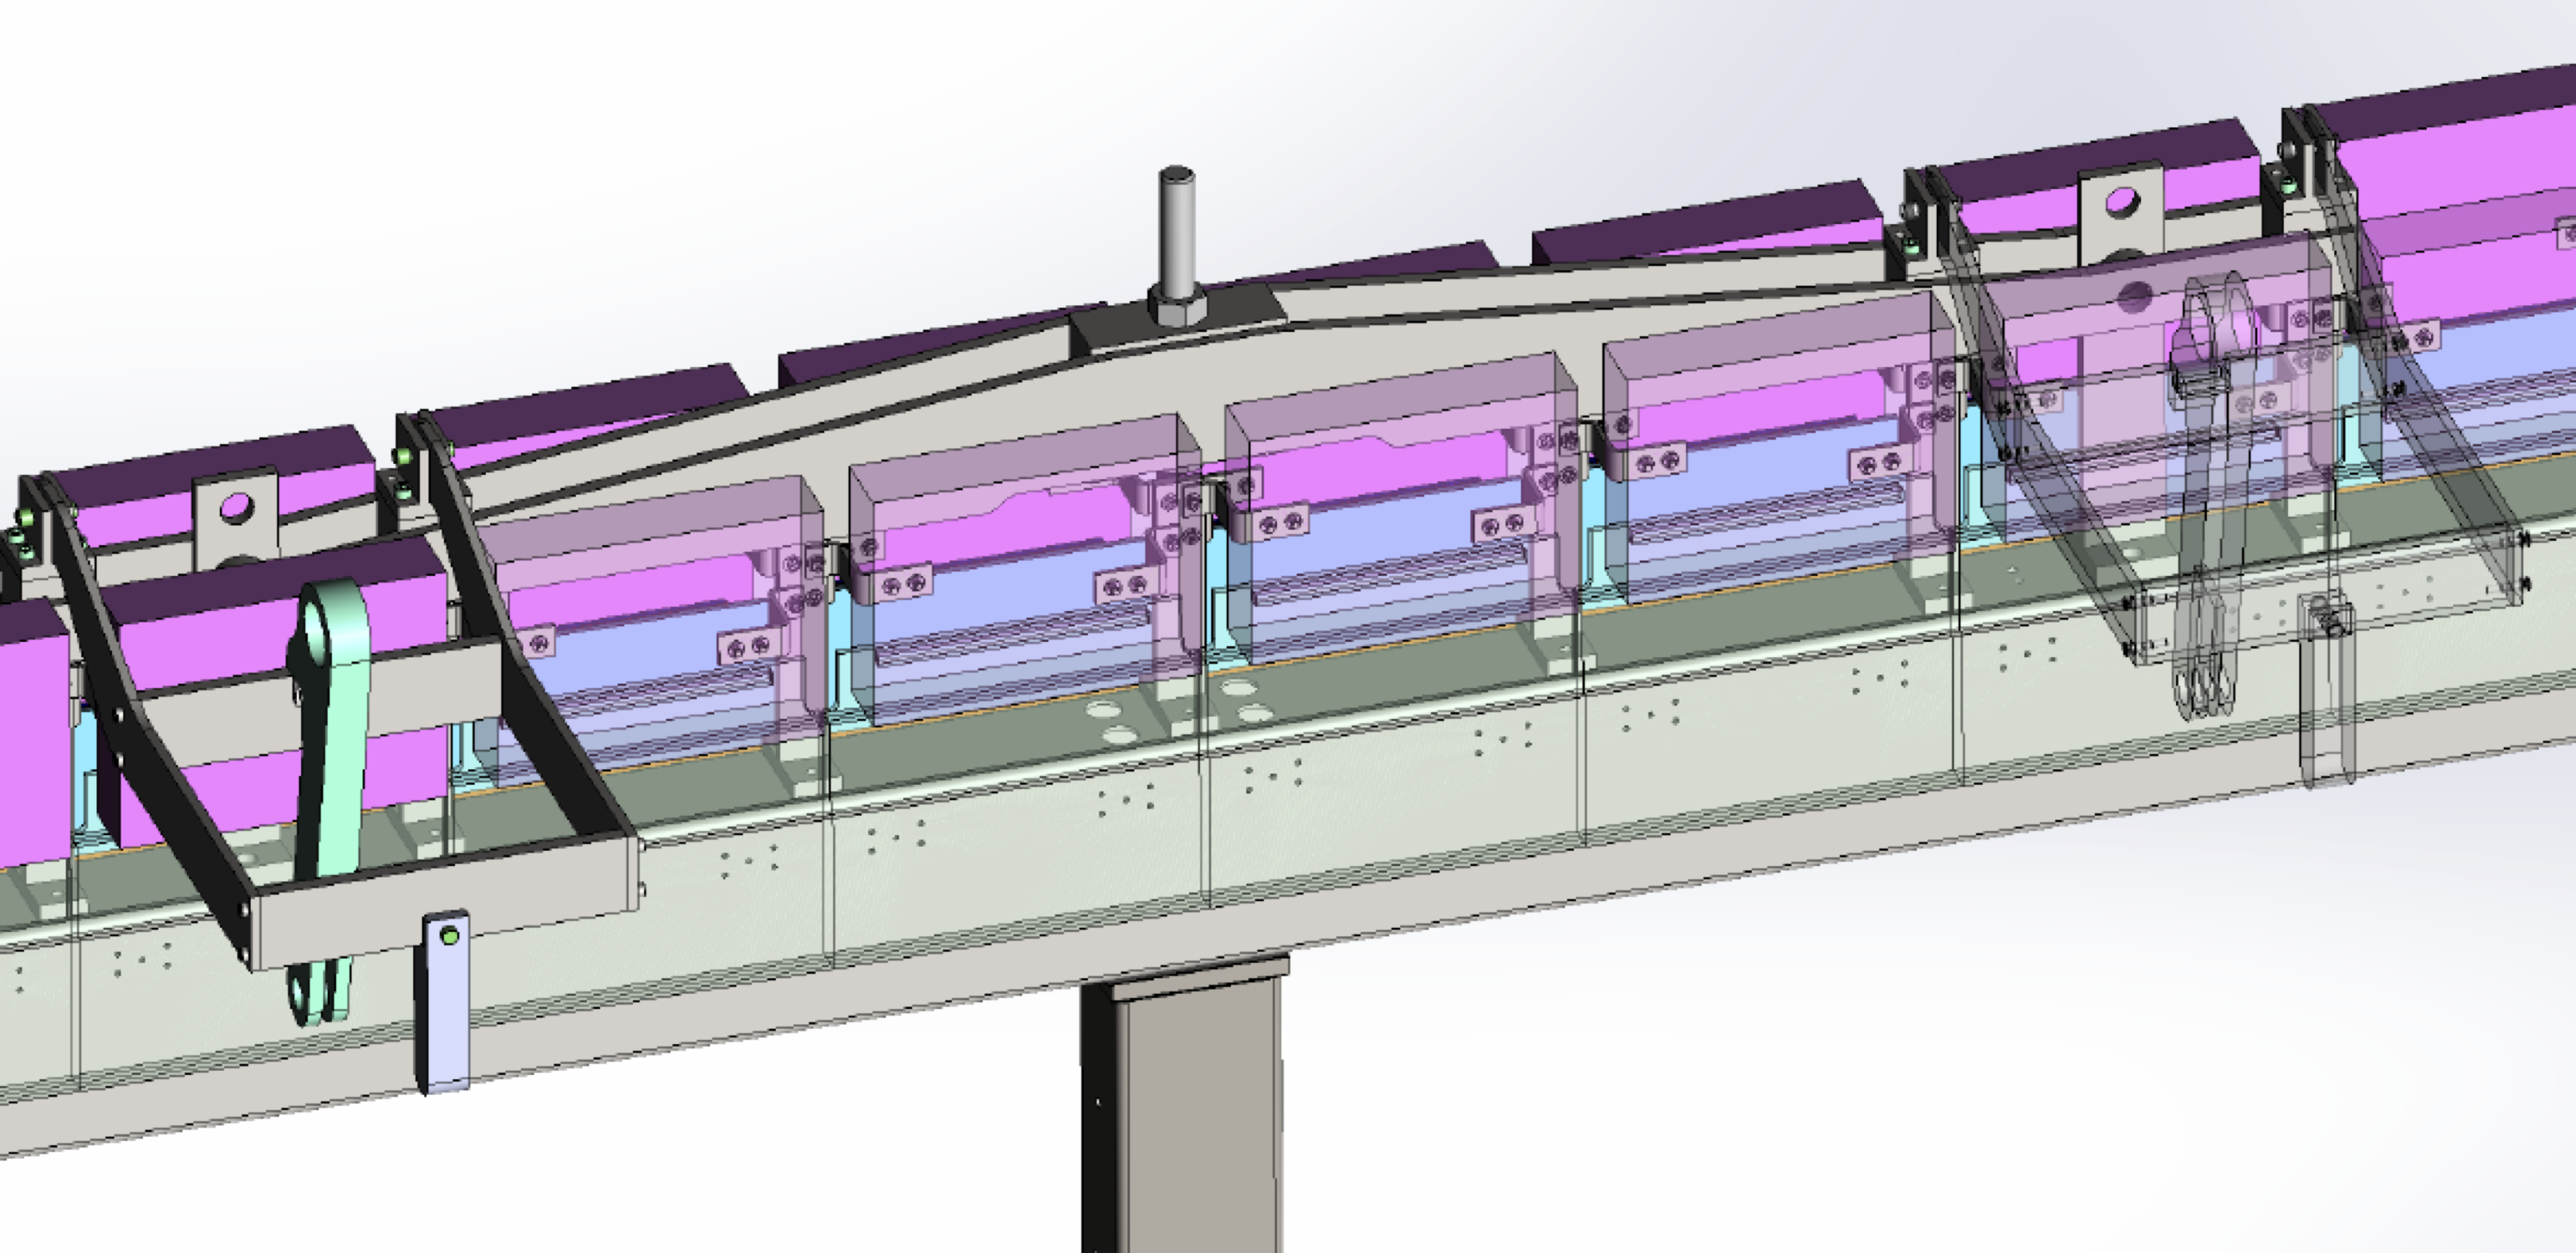
\includegraphics[width=0.9\textwidth]{figures/tpc_apa_electronicsmountingdiagram.png} 
\end{cdrfigure}

%%%%%%%%%%%%
\subsubsection{Wire supports on inner frame members - combs}

\paragraph{Purpose}

Some wire segments are long.  The longitudinal wires extend from one end of the APA to the other without going around a side -- a length of 6 m.  Even the diagonal wires across the middle of the APA are 3.9 m long.  To prevent deflection from gravity, electrostatic forces, or liquid drag from moving argon, the wires are supported at regular locations along the length of the APA.  This is done with ``combs'' mounted on each of the four cross braces that are ~ evenly spaced along the length of the APA.  This keeps the longest unsupported wire length under 1.6 m.

The nominal wire tension is 5 N but even the 1.6 m long wires could fall to 3 N of tension before the wire, held horizontally, would deviate 150 microns -- one wire diameter.  In operation the wires are either vertical or 35.7$^{\circ}$ from vertical so the actual deviation would be less.

\paragraph{Geometry}

The combs are made from 0.5 mm thick G10 with slots cut into it.  The comb for the lowest layer is glued to a base strip that's glued to the frame.  After each layer is wound another comb strip is glued to the tips of the teeth of the previous one to locate the wires in the next layer.  Each successive comb holds the previous layer of wires in the bottom of their slots (Fig. \ref{fig:tpc_apa_supportcombmodel}).

\begin{cdrfigure}[APA Support Comb Model]{tpc_apa_supportcombmodel}{A model of the combs showing how they stack.  After winding a layer the comb for the next layer is put in place.  Each comb hold the wires from the previous layer in their slots.}
\includegraphics[width=0.9\textwidth]{figures/tpc_apa_supportcombmodel.png} 
\end{cdrfigure}

Periodic holes along the length of the strip allow the use of pins to accurately locate each successive strip with the previous one.  A series of jigs are used to create and install these combs.  One jig aligns the first strip to the base strip during gluing.  Another jig locates this assembly on the frame as it is glued in place. A third jig locates each successive comb using the previously mentioned registration holes.

The wire openings in the comb stack are small enough that the wires are accurately positioned at the combs.  They are not, however, deliberately glued at the combs.  This raises the question of whether motion or vibration could cause the somewhat abrasive fiberglass comb to ``saw'' through a wire.  To address this concern we ran a test where wires were mounted on a long tube going through combs (Fig. \ref{fig:tpc_apa_wireweartestphoto}).  The tube was then mounted on a device that rotated it on its long axis.  After many more rotations than the wires will ever see, the wires were removed and examined.  No cases were found of significant erosion of the wire.  The only handling that could, possibly, yield this number of cycles would be vibration during travel.  A shipping suspension with low transmissibility at these higher frequencies will be used to prevent this kind of vibration from moving the wires against the combs

\begin{cdrfigure}[APA Wire Wear Test Photo]{tpc_apa_wireweartestphoto}{The wire wear test fixture.  The wires are confined, but not glued, in the combs mounted on this long tube.  The tube was rotated to test for wire wear from the combs.}
\includegraphics[width=0.9\textwidth]{figures/tpc_apa_wireweartestphoto.png} 
\end{cdrfigure}


%%%%%%%%%%%%
\subsubsection{APA Interconnect Features}

Some sort of constraint is needed between adjacent APAs to keep them in plane with each other.  It is also important that this constraint not apply a vertical load to adjacent APAs.  The constraint therefore takes the form of a pair of pins protruding from one edge of the APA (one high and one low on the APA) and a pair of matching slots on the other edge to engage the pins (Fig. \ref{fig:tpc_apa_pinslotdrawing}).

\begin{cdrfigure}[APA Interconnect Drawing]{tpc_apa_pinslotdrawing}{The pin/slot constraint.  The pin screws into an insert in the outside frame member of one APA and engages a slot in the outside frame member of the adjacent APA.}
\includegraphics[width=0.9\textwidth]{figures/tpc_apa_pinslotdrawing.png} 
\end{cdrfigure}

Electronic noise concerns have made it desirable to isolate APAs from each other.  To help with that this alignment pin, although it will have a steel core for strength, will have a G10 sleeve where it contacts the frame of the adjacent APA.



%\subsubsection{Integration with TPC (Dan/Jack)}

%\subsection{Wire-winding Machines (Dan)}
%
%\subsubsection{Wire wrapping concept}
%
%
%\subsubsection{Design requirements}
%
%\subsubsection{Implementation}
%\begin{itemize}
%\item{Interface frames}
%\item{Fixed APA vs. rotating APA}
%\item{Tensioning head passed around frame}
%\item{Half a layer wrapped before moving APA supports}
%\end{itemize}
%
%\subsubsection{Intermittent stop to solder}
%
%\subsubsection{Wire wrapping machinery}
%
%\subsubsection{Description/photos of machinery under construction and test}
%
%\subsubsection{Assembly sequence}
%
%\subsection{QC Procedures}
%
%\subsubsection{Quality documents (Bob, Mike Z.)}
%
%\begin{itemize}
%\item{Material certs}
%\item{Incoming inspection}
%\item{Assembly travelers}
%\end{itemize}
%
%\subsubsection{Test plan}
%
%\begin{itemize}
%\item{Wire tension}
%\end{itemize}

%\subsubsection{Assembly procedure (Lee or Dan)}

